\documentclass[12pt]{Qual}
\usepackage{preamble}

\name{Kayla Orlinsky}
\course{Complex Analysis Exam}
\term{Fall 2015}
\hwnum{Fall 2015}

\begin{document}

\begin{problem} $\,$
Evaluate the integral $$\int_0^\infty\frac{\sin^2 x}{x^2}dx$$ being careful to justify your answer.
\end{problem}


\begin{solution}$\,$
We will use ``Ol' Faithful'' the contour around the upper half plane avoiding the origin.

\begin{center}
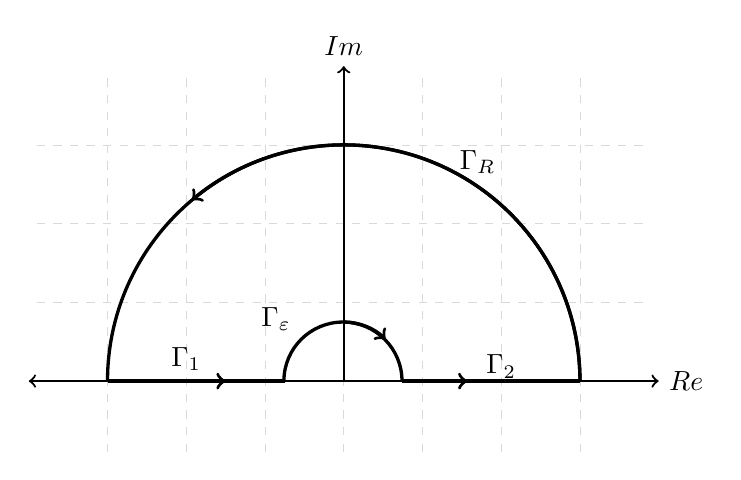
\begin{tikzpicture}
\draw[help lines, color=gray!30, dashed] (-3.9,-0.9) grid (3.9,3.9);
\draw[->,very thick] (3,0) arc (0:130:3cm);
\draw[very thick] (3,0) arc (0:180:3cm) node[above,yshift=2.5cm,xshift=4.7cm]{$\Gamma_R$};
\draw[->,very thick] (0,0.75) arc (90:45:0.75cm);
\draw[very thick] (0.74,0) arc (0:180:0.75cm) node[above,yshift=0.5cm,xshift=-0.1cm]{$\Gamma_\varepsilon$};
\draw[->,very thick] (0.74,0) -- (1.57,0);
\draw[very thick] (0.75,0) -- (3,0) node[above,yshift=-0.1cm,xshift=-1cm]{$\Gamma_2$};
\draw[->,very thick] (-3,0) -- (-1.5,0);
\draw[very thick] (-0.74,0) -- (-3,0) node[above,yshift=0cm,xshift=1cm]{$\Gamma_1$};
\draw[<->, thick] (-4,0)--(4,0) node[right]{$Re$};
\draw[->, thick] (0,0)--(0,4) node[above]{$Im$};
\end{tikzpicture}
\end{center}

Let \begin{align*}
    I_1&=\int_{\Gamma_1}\frac{1-e^{2iz}}{z^2}dz\\
    I_2&=\int_{\Gamma_2}\frac{1-e^{2iz}}{z^2}dz\\
    I_\varepsilon&=\int_{\Gamma_\varepsilon}\frac{1-e^{2iz}}{z^2}dz\\
    I_R&=\int_{\Gamma_R}\frac{1-e^{2iz}}{z^2}dz
\end{align*}

Then note that \begin{align*}
    I_1&=\int_{\Gamma_1}\frac{1-e^{2iz}}{z^2}dz\\
    &=\int_{-R}^{-\varepsilon}\frac{1-e^{2ix}}{x^2}dx\\
    &\int_R^\varepsilon-\frac{1-e^{-2ix}}{x^2}dx\\
    &=\int_\varepsilon^R\frac{1-e^{-2ix}}{x^2}dx
\end{align*}

Next, note that $$I_1+I_2=\int_\varepsilon^R\frac{2-e^{2ix}-e^{-2ix}}{x^2}dx=\int_\varepsilon^R\frac{2\left(1-\frac{e^{2ix}+e^{-2ix}}{2}\right)}{x^2}dx=2\int_\varepsilon^R\frac{1-\cos(2x)}{x^2}=4\int_\varepsilon^R\frac{\sin^2x}{x^2}dx$$

Thus, \begin{align*}
    |I_R|&=\left|\int_{\Gamma_R}\frac{1-e^{2iz}}{z^2}dz\right|\\
    &\le\int_{\Gamma_R}\frac{|1-e^{2iz}|^2}{|z|^2}dz\\
    &\le\int_0^\pi\frac{1+|e^{2iRe^{i\theta}}|}{R}d\theta\qquad z=Re^{i\theta}\\
    &=\int_0^\pi\frac{1+e^{-2R\sin\theta}}{R}d\theta\qquad 0\le\sin\theta\le1\implies e^{-2R\sin\theta}\le 1\\
    &\le\int_0^\pi\frac{2}{R}d\theta\\
    &=\frac{2\pi}{R}\to0\qquad R\to\infty
\end{align*}

Now, for $I_\varepsilon$, note that $\frac{1-e^{2iz}}{z^2}$ has an isolated pole of order $2$ at $0$. Thus, we can write $$\frac{1-e^{2iz}}{z^2}=\frac{a}{z^2}+\frac{b}{z}+f(z)$$ with $f$ analytic at $0$, $$b=\res_{z=0}\frac{1-e^{2iz}}{z^2}=\frac{d}{dz}(1-e^{2iz})\Big|_0=-2ie^{2iz}\Big|_0=-2i$$ and $$a=\lim_{z\to0}z^2\frac{1-e^{2iz}}{z^2}=\lim_{z\to0}(1-e^{2iz})=1-1=0.$$

Thus, for $\varepsilon$ small enough, \begin{align*}
    I_\varepsilon&=\int_{\Gamma_\varepsilon}\frac{1-e^{2iz}}{z^2}dz\\
    &=\int_{\Gamma_\varepsilon}\frac{-2 i}{z}+f(z)dz\\
    &=\int_\pi^02+i\varepsilon e^{i\theta}f(\varepsilon e^{i\theta})d\theta\qquad z=\varepsilon e^{i\theta}\\
    &=-2\pi +\int_\pi^0i\varepsilon e^{i\theta}f(\varepsilon e^{i\theta})d\theta\to 2\pi i\qquad \varepsilon\to0
\end{align*} since $f$ is analytic so $$\lim_{\varepsilon\to0}\int_\pi^0i\varepsilon e^{i\theta}f(\varepsilon e^{i\theta})d\theta=\int_\pi^0\lim_{\varepsilon\to0}i\varepsilon e^{i\theta}f(\varepsilon e^{i\theta})d\theta=0.$$

Finally, by the residue theorem, \begin{align*}
    0&=\lim_{R\to\infty}\lim_{\varepsilon\to0}(I_1+I_2+I_R+I_\varepsilon)\\
    &=4\int_0^\infty\frac{\sin^2x}{x^2}dx-2\pi\\
    \implies \int_0^\infty\frac{\sin^2x}{x^2}dx&=\frac{\pi}{2}
\end{align*}
\end{solution}
\newpage



\begin{problem} $\,$
Determine the number of roots of $f(z)=z^9+z^6+z^5+8z^3+1$ inside the annulus $1<|z|<2$.
\end{problem}

\begin{solution}$\,$
Let $g(z)=z^9$. Now, on \{|z|=2\} we get that \begin{align*}
    |f(z)-g(z)|&=|z^6+z^5+8z^3+1|\\
    &\le 2^6+2^5+8\cdot 2^3+1\\
    &=161\\
    &<512\\
    &=|z|^9\\
    &=|g(z)|
\end{align*} and so by Rouche's Theorem, $g$ and $f$ have the same number of zeros inside $\{|z|<2\}$ which is $9$.

Let $g(z)=8z^3$, then on $\{|z|=1\}$ \begin{align*}
    |f(z)-g(z)|&=|z^9+z^6+z^5+1|\\
    &\le 1+1+1+1\\
    &=4\\
    &<8\\
    &=8|z|^3\\
    &=|g(z)|
\end{align*}

and so by Rouche's, $f$ and $g$ have the same number of zeros inside $\{|z|<1\}$ which is $3.$

Therefore, $f$ has $9-3=6$ zeros inside the annulus $\{1<|z|<2\}.$
\end{solution}
\newpage




\begin{problem} $\,$
Suppose that $f$ is holomorphic on the open unit disk $\mathbb{D}=\{z\in\mathbb{C}:|z|<1\}$ and suppose that for $z\in\mathbb{D}$ one has $\re(f(z))>0$ and $f(0)=1.$ Prove that $|f(z)|\le\frac{1+|z|}{1-|z|}$ for all $z\in\mathbb{D}$.
\end{problem}


\begin{solution}$\,$
Since $f$ sends the unit disk to the right half plane, $if$ sends the unit disk to the upper half plane.

Thus, let $T(z)=\frac{z-i}{z+i}$. Then $T$ sends the upper half plane to the unit disk.

Furthermore, $$T(if(0))=T(i)=0$$ and so $T(if(z))$ is a map from the disk to the disk preserving the origin.

Therefore, by Schwarz' Lemma, \begin{align*}
    |T(if(z))|&\le|z|\\
    \left|\frac{if(z)-i}{if(z)+i}\right|&\le|z|\\
    \frac{|f(z)-1|}{|f(z)+1|}&\le |z|\\
    |f(z)-1|&\le |z||f(z)+1|\\
    |f(z)|-1\le |f(z)-1|&\le |z||f(z)+1|\le |z|(|f(z)|+1)\\
    (1-|z|)|f(z)|&\le 1+|z|\\
    |f(z)|&\le\frac{1+|z|}{1-|z|}
\end{align*}
\end{solution}
\newpage





\begin{problem} $\,$
For $a_n=1-\frac{1}{n^2}$, let $$f(z)=\prod_{n=1}^\infty\frac{a_n-z}{1-a_nz}.$$
\begin{enumerate}[label=(\alph*)]
    \item Show that $f$ defines a holomorphic function on the unit disk $\mathbb{D}=\{z\in\mathbb{C}:|z|<1\}.$
    \item Prove that $f$ does not have an analytic continuation to any larger disk $\{z\in\mathbb{C}:|z|<r\}$ for some $r>1$.
\end{enumerate}
\end{problem}


\begin{solution}$\,$
\begin{enumerate}[label=(\alph*)]
    \item Since $|a_n|<1$ for all $n$, $f$ defines an infinite product of analytic functions in the disk. Note that $T_n(z)=\frac{a_n-z}{1-a_nz}$ is actually an automorphism of the disk.

    Thus, $f$ is analytic in the disk if $\sum_{n=1}^\infty(T_n(z)-1)$ converges absolutely and uniformly.

    \begin{align*}
        T_n(z)-1&=\frac{a_n-z}{1-a_nz}-1\\
        &=\frac{1-\frac{1}{n^2}-z}{1-(1-\frac{1}{n^2})z}-1\\
        &=\frac{n^2-1-n^2z}{n^2-(n^2-1)z}-1\\
        &=\frac{n^2-1-n^2z}{n^2-n^2z+z}-1\\
        &=\frac{n^2-1-n^2z-(n^2-n^2z+z)}{n^2-n^2z+z}\\
        &=\frac{-z-1}{n^2-n^2z-z}\\
        &=\frac{z+1}{n^2z+z-n^2}
    \end{align*}

    Now, for all $|z|<r<1$, we have that $$|T_n(z)-1|\le \frac{|z|+1}{|z-1|n^2-|z|}<\frac{2}{(1-r)n^2-1}$$ which converges uniformly as a series. Since $r$ was arbitrary, we have that the sum converges uniformly in the unit disk.

    Thus, $f$ defines an analytic function.
    \item If $f$ has an analytic continuation at some larger disk, then $f$ must have an analytic continuation at $1$, since any larger disk will contain $1$.

    Note that $f(a_n)=0$ for all $n$, and $a_n\to 1$. Namely, if $f$ has an analytic continuation $g$ on a larger disk then $g(a_n)=0$ for all $n$ and since there is an accumulation point in any larger disk, by the identity theorem $g\equiv 0$.

    This is clearly a contradiction so $g$ cannot exist.
\end{enumerate}
\end{solution}


\end{document}
